\section{Implementierung}
Das ist der Implementierungspart

\subsection{Authentifizierung und Autorisierung}
Ein zentraler Teil bei Microservices ist die Authentifizierung sowie die Autorisierung. Es wurde sich für eine Identity Server mit OAuth2 entschieden. Die MySQL-Datenstruktur ergibt sich aus dem Datenmodell:

\begin{verbatim}
public class User
{
    [Required] public int Id { set; get; }
    public string Name { set; get; }
    public string Password { set; get; }
    public bool Active { set; get; }
    public string Role { set; get; }
}
\end{verbatim}

Als eindeutiger Identifier ist eine `Id` notwendig. Zusätzlich besitzt jeder User einen Namen, ein Passwort, ist im Standaradfall aktiviert und es wird zwischen zwei Rollen unterschieden: `customer` und  `admin`. Wie zu erwarten hat die `admin`-Rolle mehr Berechtigung als ein Customer. \\

Um den Identity Server einzurichten, müssen sogenannte NuGet-Pakete heruntergeladen werden. NuGet ist ein System, mit welchem Softwarebibliotheken bereitgestellt werden können. Diese Verweise werden zur Projektdatei hinzugefügt.

\begin{verbatim}
<PackageReference Include="IdentityServer4" Version="2.3.0" />
<PackageReference Include="IdentityServer4.AccessTokenValidation" Version="2.7.0" />
\end{verbatim}

In der `Startup.cs`, welche standardmäßig bei C\# .net vorliegt, werden grundsätzlich Serverkonfigurationen initialisiert. Dies muss für den Identity Server ebenfalls getan werden.

\begin{verbatim}
(1)
var builder = services.AddIdentityServer()
.AddInMemoryIdentityResources(Config.GetIdentityResources()) //check below
.AddInMemoryApiResources(Config.GetApis())
.AddInMemoryClients(Config.GetClients())
.AddProfileService<ProfileService>();

services.AddTransient<IResourceOwnerPasswordValidator, ResourceOwnerPasswordValidator>();
services.AddTransient<IProfileService, ProfileService>();
	
	(2)
	services.AddAuthentication("Bearer")
	.AddJwtBearer("Bearer", options =>
{
   options.Authority = "http://identity_server_service";
   [...]
   options.Audience = "srapi";
});
\end{verbatim}  

Wie man feststellen kann, sind diese Konfigurationen schon recht umfangreich, obwohl es sich in dieser Version schon um eine sehr leichtgewichtige Implementierung von OAuth2 handelt. In (1) wird der Identity Server zum Projekt hinzugefügt. Zusätzlich wird auf den `ProfileService` sowie den `ResourceOwnerPasswordValidator` verwiesen, welche anschließend initialisiert werden müssen. In (2) wird noch die `Authority` und die `Audience` gesetzt. Die `Authority` garantiert zusätzlich, dass das Token nicht von einem anderen Identity Server ausgestellt wird. Die `Audience` gibt noch einmal an, dass das ausgestellte Token nur Zugriff auf eine entsprechende `srapi`(Stirnraten-API) Ressource hat. 

\begin{verbatim}
new ApiResource("srapi", "Stirnraten API")
{
    ApiSecrets = new List<Secret>()
    {
    new Secret(CustomClientSecret.Sha256())
    }
}
\end{verbatim}

Zusätzlich müssen noch die beiden in den Grundlagen erwähnten Flows (`ClientCredentials` und `ResourceOwnerPassword`) implementiert werden. 

\begin{verbatim}{
[...]
new Client
{
    ClientId = CustomClientId,
    AllowedGrantTypes = GrantTypes.ClientCredentials,
    ClientSecrets =
    {
    new Secret(CustomClientSecret.Sha256())
    },
    AllowedScopes =
    {
    "srapi"
    }
},

new Client
{
    ClientId = "sr.client",
    AllowedGrantTypes = GrantTypes.ResourceOwnerPassword,
    ClientSecrets =
    {
    new Secret("secret".Sha256())
    },
    AllowedScopes =
    {
    "srapi"
    }
}

\end{verbatim}

Durch diese Flows ist garantiert, dass die API grundsätzlich geschützt ist, d.h. auch dann wenn Benutzer keine Benutzerdaten hinterlegt haben. Werden allerdings benutzerspezifische Zugänge hinterlegt, erhalten diese noch mehr Zugriffsrechte auf die API. Dies wird im Bereich \ref{sec:umsetzung_api_gateway} deutlich. \\

Wenn eine Anfrage mit Benutzernamen und Passwort gestellt wird, ruft der Identity Server in seinem Abarbeitungszyklus folgende Methode ab: 

\begin{verbatim}
public async Task ValidateAsync(ResourceOwnerPasswordValidationContext context)
		{
		(1)
		var user = await _unitOfWork.UserRepository.GetUserByNameAndPasswordAsync(context.UserName,
		context.Password);
		
		(2)
		if (user == null)
		{
		context.Result = new GrantValidationResult(
		TokenRequestErrors.InvalidGrant,
		"invalid custom credential");
		return;
		}
		
		if (!user.Active)
		{
		context.Result = new GrantValidationResult(
		TokenRequestErrors.InvalidClient,
		"User was deactivated by admin");
		return;
		}
		
		(3)
		context.Result = new GrantValidationResult(
		subject: user.Id.ToString(),
		authenticationMethod: "custom",
		claims: GetUserClaims(user)); //get user claims
		}
\end{verbatim}

In (1) wird ein Benutzer gesucht, welcher mit dem übergebenen Namen und Passwort übereinstimmt. In (2) wird dieser validiert und in (3) das Token anhand der `Claims` generiert. `Claims` sind vereinfacht ausgedrückt, zusätzlich Informationen, welche man in dem Token übergeben möchte. 

\begin{verbatim}
return new[]
{
new Claim("user_id", user.Id.ToString() ?? ""),
new Claim(JwtClaimTypes.Name, user.Name),
new Claim(JwtClaimTypes.Role, user.Role)
};
\end{verbatim}

In der umgesetzten API wird eine `user\_id`, der `Name` sowie die `Role` übergeben. Alles wird ggf. von anderen Microservices benötigt, um eine entsprechende Autorisierung zu gewährleisten.\\

Abbildung \ref{fig:client_credentials_flow} und \ref{fig:password_flow} zeigen wie über eine POST Abfrage die entsprechenden Token ausgestellt werden können.\\

\begin{figure}[ht]
	\centering
	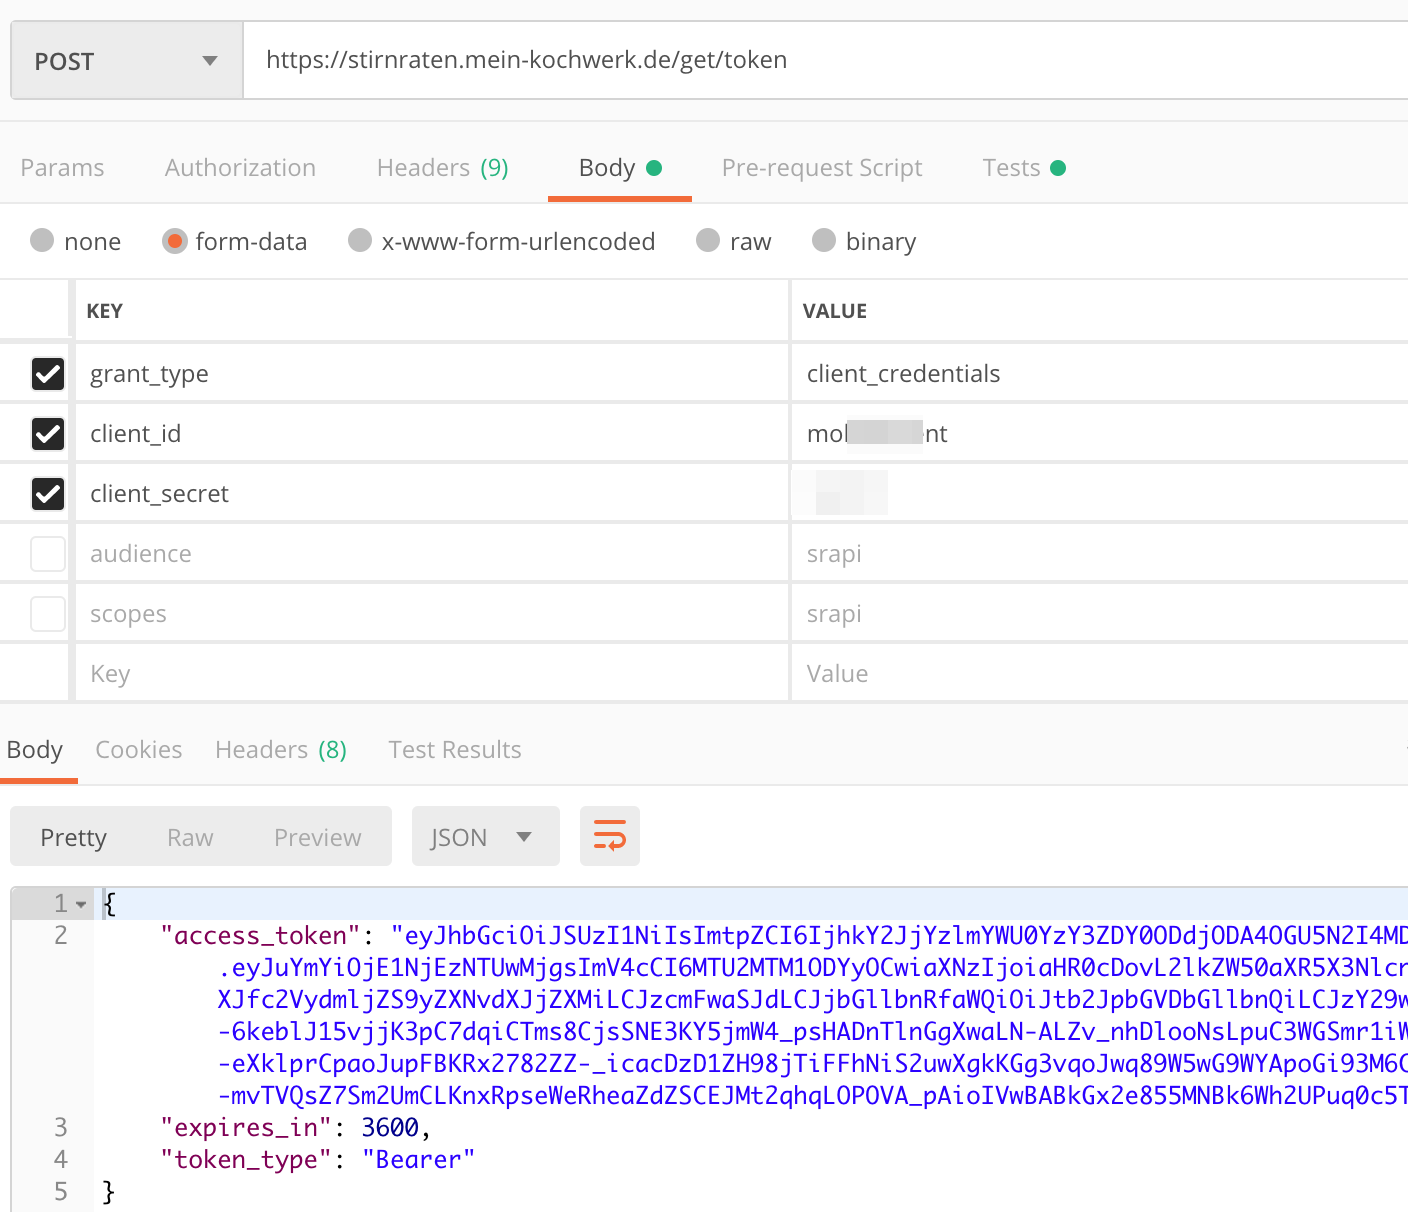
\includegraphics[width=0.6\textwidth]{client_credentials_flow}
	\caption[Über Postman gesendeter Client Credential Flow] {Über Postman gesendeter Client Credential Flow. Mit Hilfe dieses Tokens erhält man für 3600 Sekunden (eine Stunde) beschränkten Zugang zur API, um  z.B. Kategorien abzurufen, neue Wörter einzusenden oder ein Benutzerkonto anzulegen.}
	\label{fig:client_credentials_flow}
\end{figure} 

\begin{figure}[!ht]
	\centering
	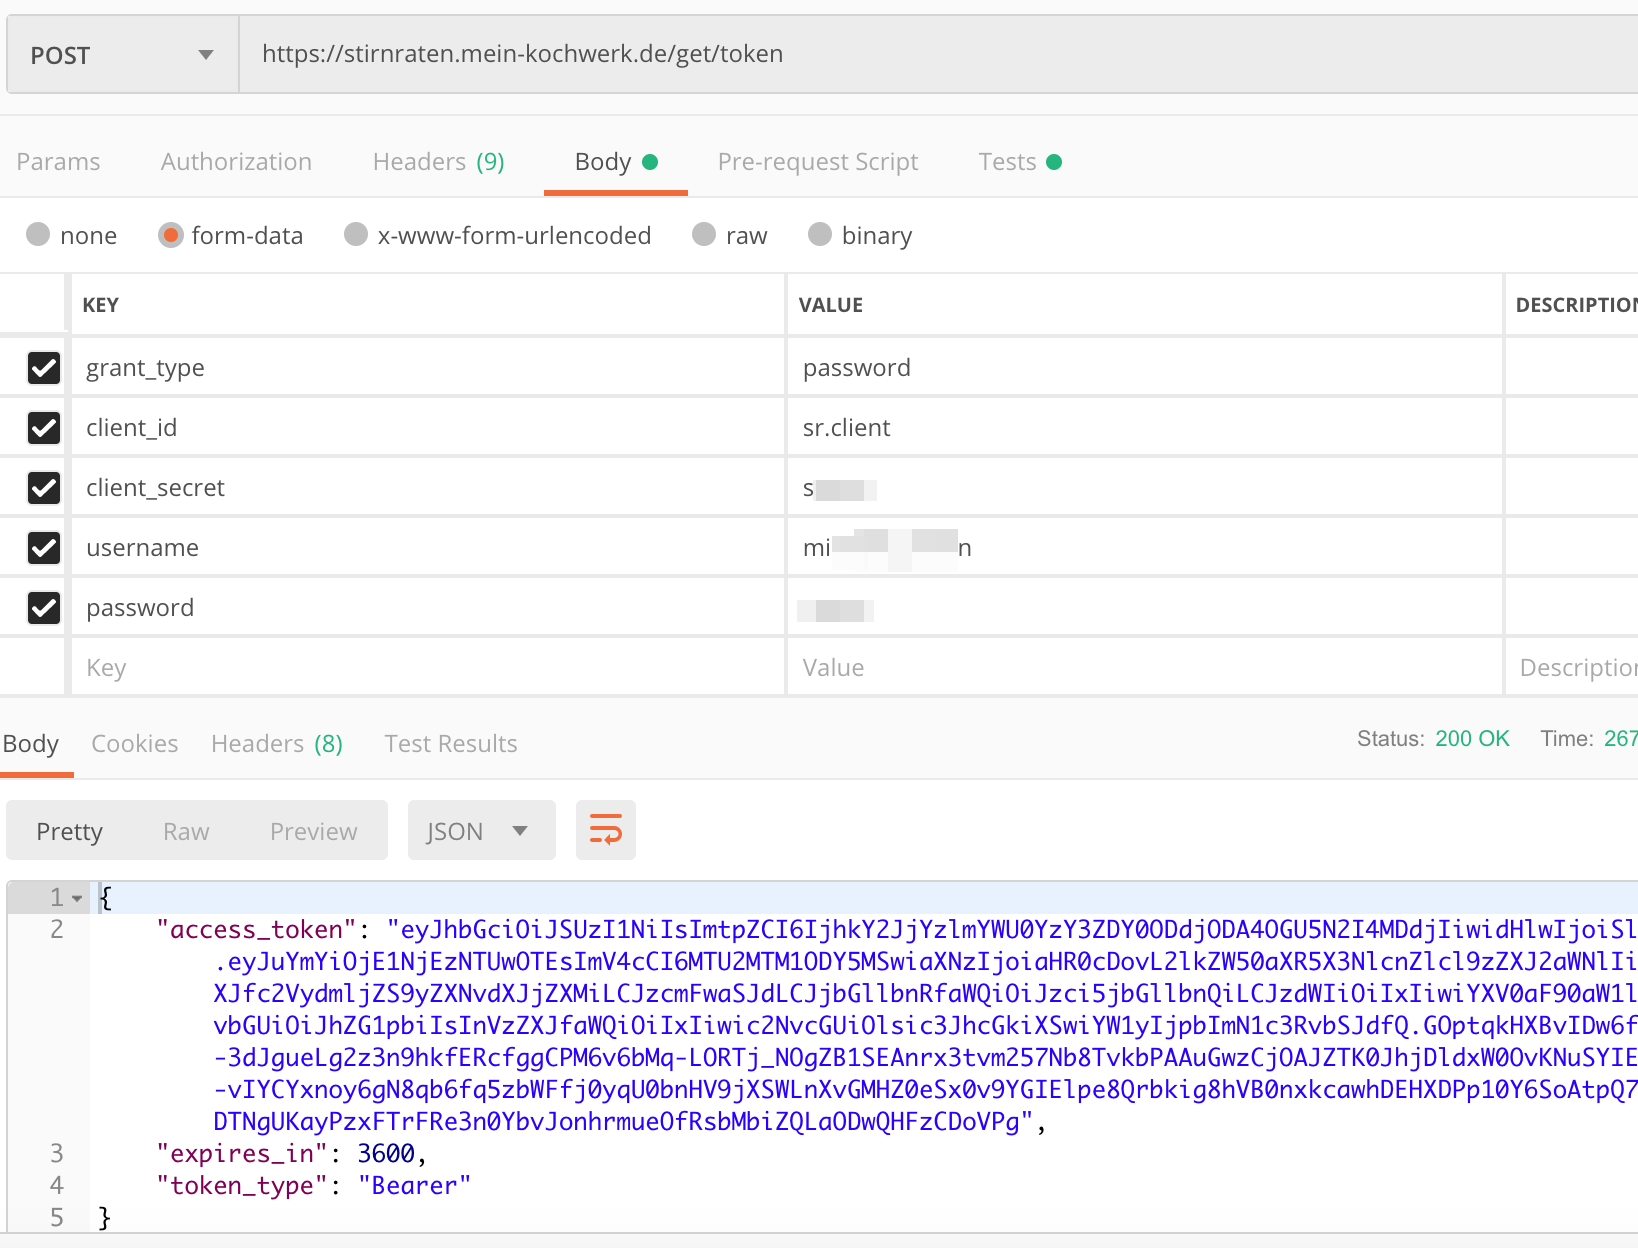
\includegraphics[width=0.6\textwidth]{password_flow}
	\caption[Über Postman gesendeter Password Flow] {Über Postman gesendeter Password Flow. Er ist ebenfalls 3600 Sekunden lang gültig und hat mehr Berechtigung, wie z.B. das Speichern eines Benutzerprofils.}
	\label{fig:password_flow}
\end{figure} \\

Enkodiert sieht so ein ausgestellter Benutzer-Token wie folgt aus: \\

\begin{verbatim}
		[...]
		"iss": "http://identity_server_service",
		"aud": [
		"http://identity_server_service/resources",
		"srapi"
		],
		"client_id": "sr.client",
		[...]
		"role": "admin",
		"user_id": "1",
		"scope": [
		"srapi"
		],
		"amr": [
		"custom"
		]
		[...]
\end{verbatim}  

Durch diese Informationen kann das API-Gateway bereits eine Autorisierung vornehmen. Wie dies im Detail funktioniert, wird im Abschnitt \ref{umsetzung_api_gateway} deutlich. 

\subsection{Umsetzung API-Gateway}\label{sec:umsetzung_api_gateway}

\subsection{Asynchrone  Kommunikation}
// ieine Queue umsetzen (RabbitMQ, Kafka...)

\subsection{Service Architektur}
// nginx vom Hoster
// deployment
// Grafik erstellen, welche Services es gibt und wie diese Kommunizieren 
// Docker erwähnen und Beispiel einfügen




